\section{Bewegungen}
%
%
%
\subsubsection{Definition:}
Eine Abbildung heißt Bewegung oder Isometrie wenn $\forall a,b \in \mathbb{R}^{2}\qquad \Vert A(a) - A(b) \Vert = \Vert \vec{a}-\vec{b}\Vert$.
%
%
%
\subsubsection{Satz:}
$A: \mathbb{R}^{2} \rightarrow \mathbb{R}^{2}$ Bewegung mit $A\begin{pmatrix} 0 \\ 0 \end{pmatrix} = \begin{pmatrix} 0 \\ 0 \end{pmatrix}$. Dann ist $A$ linear. Es gibt $c,s \in \mathbb{R}$ mit $c^{2}+s^{2}=1$, sodass die Matrix von $A$ durch $R_{c,s} = \begin{pmatrix} c & -s \\ s & c \end{pmatrix} \, det(R_{c,s}) = 1$ oder $S_{c,s} = \begin{pmatrix} c & s \\ s & -c \end{pmatrix} \, det(S_{c,s}) = -1$ gegeben ist.
%
\begin{figure}[H]
\centering

\includegraphics[width=0.75\textwidth]{mainmatter/chapter1/pics/bewegung.png}
\end{figure}
%
\subsubsection{Beweis:}
$A$ ist Isometrie.\\
$A\begin{pmatrix} 1 \\ 0 \end{pmatrix} = \begin{pmatrix} c \\ s \end{pmatrix}  \quad A\begin{pmatrix} 0 \\ 1 \end{pmatrix} = \begin{pmatrix} t \\ u \end{pmatrix} \quad A\begin{pmatrix} x \\ y \end{pmatrix} = \begin{pmatrix} z \\ w \end{pmatrix}$\\
$ c^{2}+s^{2}=1=t^{2}+u^{2}$\\
$(c-t)^{2} + (s-u)^{2} = 2 =2-2\mathop{\underbrace{(tc+su)}}\limits_{\Rightarrow 0 }$ weil der Abstand von $\begin{pmatrix} 1 \\ 0 \end{pmatrix}$ zu $\begin{pmatrix} 0 \\ 1 \end{pmatrix}$ gleich $\sqrt{2}$ ist. \\
$\Rightarrow \begin{pmatrix} t \\ u \end{pmatrix} = \lambda \begin{pmatrix} -s \\ c \end{pmatrix}, \lambda = \pm 1$ somit $ t = -s, \, u = c$ oder $t=s \, u =-c$\\
$A$ linear: z.z. $\begin{pmatrix}z \\ w \end{pmatrix} = \begin{pmatrix} cx \mp sy \\ sx \pm cy \end{pmatrix}$\\
Fall $\begin{pmatrix} 0 \\ 1 \end{pmatrix} \mapsto \begin{pmatrix} -s \\ c \end{pmatrix}$\\
$x^{2}+y^{2} = z^{2} + w^{2}$\\
$(x-1)^{2} + y^{2} \mathop{=}\limits^{\text{\RM{1}}} ( z-c)^{2} + (w-s)^{2}$\\
$\Leftrightarrow x^{2}-2x+1+y^{2} = z^{2}-2zc+c^{2}+w^{2}-2sw+s^{2}$\\
$\Rightarrow x= cz + sw$\\
$(z+s)^{2} + (w-c)^{2} = x^{2}+(y-1)^{2}$\\
$\Leftrightarrow 2sz-2cw = -2y$\\
$\Rightarrow y = -sz$\\
$\begin{pmatrix} c & -s \\ s & c \end{pmatrix} \quad \begin{pmatrix} c & s \\ -s & c \end{pmatrix} \quad \begin{pmatrix} z \\ w \end{pmatrix} = \begin{pmatrix} x \\ y \end{pmatrix}$ \\
$(R_{c,s} = \begin{pmatrix} c & -s \\ s & c \end{pmatrix}, \, S_{c,s} = \begin{pmatrix} c & s \\ s & -c \end{pmatrix})$\\
%
%
%
\subsubsection{Idee:}
Spiegelung ges: $\vec{a}: A(\vec{a})=\vec{a}$
%
%
%
\subsubsection{Fall \RM{1}:} 
$
\left\{
\begin{array}{c l}     
    cx-sy=x  & s \neq 0 \text{ sonst } \begin{pmatrix} 1 \\ 0 \end{pmatrix}= \begin{pmatrix} c \\ s \end{pmatrix}, x \neq q \text{ (trivial)}\\
    sx+cy = y &
\end{array}\right.
\Leftrightarrow
\left\{
\begin{array}{c l}     
 (c-1)x - sy = 0 & \mathop{\Rightarrow}\limits^{s\neq 0} y = \frac{c-1}{s}x \\
    sx + (c-1)y=0 & \mathop{\Rightarrow}\limits^{:x} s + \frac{(c-1)^{2}}{s}=0
\end{array}\right.$\\
\quad\\
$1-x^{2} + (c-1)^{2} = 0 \Rightarrow 2 = 2c, \, c=1\Rightarrow s = 0 \qquad\lightning$
%
%
%
\subsubsection{Fall \RM{2}:}
$\begin{cases} 
cx + sy = x  \\ 
sx -cy = y
\end{cases}
\Rightarrow $2. Gleichung ist Folge der ersten wenn $s = 0 \Rightarrow c = 1$ wir erhalten $\begin{pmatrix} 1 & 0 \\ 0 & -1 \end{pmatrix}$: $x$-Achsen-Spiegelung\\
$s \neq 0: y = \frac{1-c}{s}x\rightarrow s^{2} = (1+c)(1-c)\Rightarrow y=\frac{s}{1+c}x$ Diese wird gelöst von\\
$\begin{pmatrix} x \\ y \end{pmatrix} = \begin{pmatrix} c+1 \\ s \end{pmatrix}$ und skalare Vielfache. Noch zz., dass $R$ und $S$ Isometrien sind:\\
$\Vert A(\vec{a})\Vert^{2} = (cx-sy)^{2}+(sx+cy)^{2} = c^{2}x^{2}-2cxsy+s^{2}y^{2}+s^{2}x^{2}+2cxsy + c^{2} y^{2} = x^{2}+y^{2}=\Vert\vec{a}\Vert^{2}$ also längenerhaltend /* $\vec{a}=\begin{pmatrix} x \\ y \end{pmatrix}$*/\\
somit $\Vert A(\vec{a})-A(\vec{b})\Vert = \Vert A(\vec{a}-\vec{b})\Vert = \Vert \vec{a}-\vec{b}\Vert$ abstandserhaltend !\\
%
%
%
\subsubsection{Satz:}
\begin{enumerate}
	\item Das Produkt zweier Spiegelungen ist eine Drehung.
	\item Jede Drehung lässt sich als Produkt zweier Spiegelungen beschreiben.
\end{enumerate}
\begin{enumerate}
	\item $ \begin{pmatrix} a & b \\ b & -a \end{pmatrix}  \begin{pmatrix} c & d \\ d & -c \end{pmatrix} = \begin{pmatrix} ac+bd & ad-bc \\ bc-ad & bd+ac \end{pmatrix} \Rightarrow$ von Typ $ \begin{pmatrix} c & -s \\ s & c \end{pmatrix} = R_{c,s}$
	\item $\begin{pmatrix} -s & c \\ c & s \end{pmatrix} \begin{pmatrix} 0 & 1 \\ 1 & 0 \end{pmatrix} = \begin{pmatrix} c  & -s \\ s & c \end{pmatrix}$
\end{enumerate}
%
%
%
\subsubsection{Satz:}
Die Verknüpfung zweier Drehungen ist einer Drehung und die Inverse einer Drehung ist eine Drehung. 
%
\begin{figure}[H]
\centering
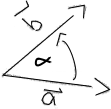
\includegraphics[width=0.1\textwidth]{mainmatter/chapter1/pics/bewegung2.png}
\end{figure}
%
\subsubsection{Beweis:}
$R_{c,s} \cdot R_{t,u}=R_{ct-su,cu+st}=R_{t,u} \cdot R_{c,s} \Leftrightarrow R_{t,u}\textrm{ ist vertauschbar mit } R_{c,s}$ \\
$R_{c,s}\cdot R_{c,-s} = R_{1,0} = Id$\\
%
%
%
\subsubsection{Satz:}
$\vec{a} \neq \vec{0} \neq \vec{b}$, gibt es eindeutig bestimmtes $\lambda \in \mathbb{R}:$\\
Drehung $ R(\vec{a})=\lambda \cdot b$\\
$R(\vec{0})=\vec{0}$\\
%
\begin{figure}[H]
\centering

\includegraphics[width=0.3\textwidth]{mainmatter/chapter1/pics/bewegung3.png}
\end{figure}
%
Existenz $\mathop{\Rightarrow}\limits^{\text{!}}$ Eindeutigkeit\\
$R\begin{pmatrix} t \\ u \end{pmatrix} = \begin{pmatrix} c \\ s \end{pmatrix}$\\
$T:= R_{c,-s} \, R \, R_{tu}$ ist Drehung mit\\
$T\begin{pmatrix} 1 \\ 0 \end{pmatrix} = \begin{pmatrix} 1 \\ 0 \end{pmatrix}$\\
$\Rightarrow R = R_{cs} \circ R_{t-u} \Rightarrow$ Eindeutigkeit \\
$R:= R_{cs} \circ R_{t-u}$\\
$R(\vec{a}) = R_{cs} \circ R_{t-u} (\vec{a}) = R_{c,s} \Vert a \Vert \begin{pmatrix} 1 \\ 0 \end{pmatrix} = \frac{\Vert \vec{a}\Vert \vec{b}}{\Vert \vec{b} \Vert}$
%
%
%
